 %
% In principle, this file can be redistributed and/or modified under
% the terms of the GNU Public License, version 2.
%
% However, this file is supposed to be a template to be modified
% for your own needs. For this reason, if you use this file as a
% template and not specifically distribute it as part of a another
% package/program, I grant the extra permission to freely copy and
% modify this file as you see fit and even to delete this copyright
% notice. 

\documentclass[9pt]{beamer}
 \usepackage{multirow}
 \usepackage{natbib}
 \usepackage[normalem]{ulem}
 \useunder{\uline}{\ul}{}
 \usepackage[utf8]{inputenc}
\usepackage{mathtools}
\usepackage{IEEEtrantools}
\usepackage[english,brazil]{babel}
\definecolor{maroon}{RGB}{153, 0, 0}
\usepackage[colorlinks=true, linkcolor= black, citecolor=maroon]{hyperref}


% There are many different themes available for Beamer. A comprehensive
% list with examples is given here:
% http://deic.uab.es/~iblanes/beamer_gallery/index_by_theme.html
% You can uncomment the themes below if you would like to use a different
% one:
%\usetheme{AnnArbor}
%\usetheme{Antibes}
%\usetheme{Bergen}
%\usetheme{Berkeley}
%\usetheme{Berlin}
%\usetheme{Boadilla}
%\usetheme{boxes}
%\usetheme{CambridgeUS}
%\usetheme{Copenhagen}
%\usetheme{Darmstadt}
%\usetheme{default}
%\usetheme{Frankfurt}
%\usetheme{Goettingen}
%\usetheme{Hannover}
%\usetheme{Ilmenau}
%\usetheme{JuanLesPins}
%\usetheme{Luebeck}
\usetheme{Madrid}
\definecolor{UBCblue}{rgb}{0.04706, 0.13725, 0.26667} % UBC Blue (primary)


\usecolortheme[named=UBCblue]{structure}
%\usetheme{Malmoe}
%\usetheme{Marburg}
%\usetheme{Montpellier}
%\usetheme{PaloAlto}
%\usetheme{Pittsburgh}
%\usetheme{Rochester}
%\usetheme{Singapore}
%\usetheme{Szeged}
%\usetheme{Warsaw}
\usepackage[utf8]{inputenc}
\usepackage{booktabs}
\let\olditem\item
\renewcommand{\item}{%
\olditem\vspace{\fill}} 
\usepackage{graphicx}
\usepackage{xfrac}
\usepackage{amsmath,amssymb,hyperref,array,xcolor,multicol,verbatim,mathpazo}

\setbeamertemplate{theorems}[numbered]

%\makeatother
%\setbeamertemplate{footline}
%{
  %\leavevmode%
  %\hbox{%
  %\begin{beamercolorbox}[wd=.3\paperwidth,ht=2.25ex,dp=1ex,center]{author in head/foot}%
   % \usebeamerfont{author in head/foot}\insertshortauthor
  %\end{beamercolorbox}%
  %\begin{beamercolorbox}[wd=.7\paperwidth,ht=2.25ex,dp=1ex,center]{title in head/foot}%
    %\usebeamerfont{title in head/foot}\insertshorttitle\hspace*{3em}
   % \insertframenumber{} / \inserttotalframenumber\hspace*{1ex}
  %\end{beamercolorbox}}%
 % \vskip0pt%
%}
%

\makeatletter
\setbeamertemplate{navigation symbols}{}
\title{Taxa Natural de Juros no Brasil: uma abordagem DSGE}
\subtitle{} 
\author[Renan Alves]{ Renan Alves e Marcelo Kfoury}
\date{\today}

\begin{document}
\setbeamertemplate{caption}{\raggedright\insertcaption\par}
\maketitle


%%%%%%%%%%%%%%%%%%%%%%%%%%%%%%%%%%%%%%%%%%%%%%%%%%%%%%%%%%%%%%%%%%%%%%%%%%%%
%%%%%%%%%%%%%%%%%%%%%%%%%%%%%%%%%%%%%%%%%%%%%%%%%%%%%%%%%%%%%%%%%%%%%%%%%%%%
\begin{frame}{Introdução}
\begin{itemize}

\item O banqueiro central ao direcionar a política monetária avalia o comportamento da economia em relação a algum parâmetro que ele segue como referência (\textit{benchmark}) 

\item A taxa de juros nominal determinada pelo banco central oscila ao redor deste \textit{benchmark}, o qual não é observado de forma direta nos dados. Esse referencial é chamado de taxa natural de juros

\item A taxa natural de juros é uma variável chave para o Banco Central, pois esta é vista como uma taxa de equilíbrio

\item O objetivo do artigo é estimar a taxa natural de juros, para a economia brasileira, por meio de um modelo Novo Keynesiano

\item O modelo incorpora as principais características dos modelos DSGE de pequena economia aberta e possibilita investigar como choques externos afetam a taxa natural no Brasil, durante o período pós metas de inflação


\end{itemize}
\end{frame}
%%%%%%%%%%%%%%%%%%%%%%%%%%%%%%%%%%%%%%%%%%%%%%%%%%%%%%%%%%%%%%%%%%%%%%%%%%%%
%%%%%%%%%%%%%%%%%%%%%%%%%%%%%%%%%%%%%%%%%%%%%%%%%%%%%%%%%%%%%%%%%%%%%%%%%%%%
\begin{frame}{Taxa natural de juros}
\begin{itemize}

\item Um \textit{benchmark} importante para o policymaker é como a economia estaria se por acaso não houvesse rigidez de preços, ou seja, preços totalmente flexíveis

\item Taxa natural de juros e nível natural do produto (ou potencial), quando preços e salários são flexíveis. A política monetária é formulada em termos de desvios dessas taxas naturais, logo em termos de hiato do produto e hiato da taxa de juros

\item É um indicador fundamental de uma apropriada política monetária, em especial em um regime de metas de inflação

\item É adequado ter uma boa estimativa dela e consequentemente do hiato da taxa de juros, para indicar se a política monetária adotada foi contracionista ou expansionista

\end{itemize}
\end{frame}
%%%%%%%%%%%%%%%%%%%%%%%%%%%%%%%%%%%%%%%%%%%%%%%%%%%%%%%%%%%%%%%%%%%%%%%%%%%%
%%%%%%%%%%%%%%%%%%%%%%%%%%%%%%%%%%%%%%%%%%%%%%%%%%%%%%%%%%%%%%%%%%%%%%%%%%%%
\begin{frame}{Como os economistas estimam Taxa Natural de Juros?}
\begin{itemize}

\item O maior problema encontrado na literatura é que a taxa neutra de juros não é observada. Por conta disso, diversas técnicas econométricas são utilizadas para estimar a taxa natural de juros 

\item Laubach e Williams (2003) a taxa natural de juros é uma variável latente que depende da taxa de crescimento da tendência do produto potencial e uma raiz unitária que captura outros determinantes. A taxa natural é inferida a partir da relação estrutural que conecta o hiato do produto, a inflação e os desvios da taxa real de juros do seu nível natural. Modelos dessa família são chamados de semi estruturais

\item A segunda classe de artigos utiliza modelos estruturais para estimar a taxa neutra de juros. Estes são conhecidos por modelos de equilíbrio geral dinâmicos estocásticos (DSGE)

\item Modelos DSGE apresentam diversas fricções nominais, como rigidez de salários e preços, fricções reais, como formação de hábito, custo de ajustamento do capital, nível de utilização da capacidade, além de vários choques estruturais, como choques de produtividade, eficiência marginal do investimento, markup de preços e salários.

\end{itemize}
\end{frame}
%%%%%%%%%%%%%%%%%%%%%%%%%%%%%%%%%%%%%%%%%%%%%%%%%%%%%%%%%%%%%%%%%%%%%%%%%%%%
%%%%%%%%%%%%%%%%%%%%%%%%%%%%%%%%%%%%%%%%%%%%%%%%%%%%%%%%%%%%%%%%%%%%%%%%%%%%
\begin{frame}{Modelo}
\begin{itemize}

\item Modelo é Gali e Monacelli (2005) com Lubik e Schorfheide (2007) 

\item Curva IS para pequena economia aberta:

\begin{equation*}
    x_t = E_t(x_{t+1}) - \frac{1}{(1-\alpha)\tau_{\alpha}}\left(i_t - E_t(\pi_{t+1}) - r_t^{n} \right)
\end{equation*}

$\tau_{\alpha} = \frac{1}{\tau + \alpha(2 - \alpha)(\eta - \tau)}$.

\item Hiato do produto $x_t = y_{A,t} - y_{A,t}^{n}$ e a taxa natural real de juros $r_t^{n}$.

\item O produto potencial doméstico $y_{A,t}^{n}$ depende do produto do resto do mundo $y_{A,t}^{f}$ que segue: $y_{A,t}^{n} = - \Gamma_{*}y_{A,t}^{f} $.

onde $\Gamma_{*}=1-\sigma^{-1} \tau_{\alpha} / \sigma^{-1} \tau_{\alpha}+\sigma^{-1} \varphi$


\end{itemize}
\end{frame}
%%%%%%%%%%%%%%%%%%%%%%%%%%%%%%%%%%%%%%%%%%%%%%%%%%%%%%%%%%%%%%%%%%%%%%%%%%%%
%%%%%%%%%%%%%%%%%%%%%%%%%%%%%%%%%%%%%%%%%%%%%%%%%%%%%%%%%%%%%%%%%%%%%%%%%%%%
\begin{frame}{Modelo}
\begin{itemize}
\item A taxa natural real de juros $r_t^{n}$ é dada por:
\begin{equation*}
    r_t^{n} = E_t(\Delta \varepsilon_{t+1}^{c}) + \left( \frac{1 + \phi}{1 + \tau \phi} \right)E_t(z_{t+1}) + \left[\frac{1}{\tau} -(1 - \alpha)\tau_{\alpha}(\Gamma_{*}+1)   \right]E_t(\Delta y_{A,t+1}^{f})
\end{equation*}

\item choque de preferencia: $\varepsilon_{t+1}^{c}$, choque de tecnologia $z_t = ln\left( \frac{A_t}{A_{t-1}} \right)$.

\item A curva de NKPC:

\begin{equation*}
    \pi_t = \beta E_t(\pi_{t+1} ) + \alpha \beta E_t(q_{t+1}) - \alpha \Delta q_t + (\tau_{\alpha} + \phi) \kappa x_t + u_t
\end{equation*}

\item os termos de troca $q_t$. A inflação: $\pi_t = \Delta s_t + (1 - \alpha) \Delta q_t + \pi_t^{f} $. $\pi_t^{f}$ é a inflação do resto do mundo e segue um AR(1). 


\end{itemize}
\end{frame}
%%%%%%%%%%%%%%%%%%%%%%%%%%%%%%%%%%%%%%%%%%%%%%%%%%%%%%%%%%%%%%%%%%%%%%%%%%%%
%%%%%%%%%%%%%%%%%%%%%%%%%%%%%%%%%%%%%%%%%%%%%%%%%%%%%%%%%%%%%%%%%%%%%%%%%%%%
\begin{frame}{Modelo}
\begin{itemize}
\item 3 regras de juros diferentes.

\item A regra de Taylor convencional:
\begin{equation*}
    i_t = \rho_i i_{t-1} + (1 - \rho_i)(\psi_{x}x_t + \psi_{\pi} \pi_t) + \varepsilon_{i,t}
\end{equation*}

\item Regra Wickseliana (seguindo Cúrdia, V., Ferrero, A., Ng, G. C., & Tambalotti, A. (2015).):
\begin{equation*}
    i_t = \rho_i i_{t-1} + (1 - \rho_i)(r_t^{n} + \psi_{\pi} \pi_t) + \varepsilon_{i,t}
\end{equation*}

\item Regra Wickseliana e Taylor (seguindo Cúrdia, V., Ferrero, A., Ng, G. C., & Tambalotti, A. (2015).):
\begin{equation*}
    i_t = \rho_i i_{t-1} + (1 - \rho_i)(r_t^{n} + \psi_{x}x_t + \psi_{\pi} \pi_t) + \varepsilon_{i,t}
\end{equation*}

\item A taxa de crescimento dos termos de troca é dado por: $\Delta q_t = \tau_{\alpha}(\Delta y_{A,t}^{f} - \Delta y_{A,t})$.

\item A taxa de crescimento dos termos de troca segue um AR(1):$\Delta q_t = \rho_q \Delta q_{t-1} + \varepsilon_{q,t}$.


\end{itemize}
\end{frame}
%%%%%%%%%%%%%%%%%%%%%%%%%%%%%%%%%%%%%%%%%%%%%%%%%%%%%%%%%%%%%%%%%%%%%%%%%%%%
%%%%%%%%%%%%%%%%%%%%%%%%%%%%%%%%%%%%%%%%%%%%%%%%%%%%%%%%%%%%%%%%%%%%%%%%%%%%
\begin{frame}{Base de Dados}
\begin{itemize}
    \item A amostra começa em janeiro de 2000 e vai até o dezembro de 2019
    
    \item As variáveis domésticas: PIB, inflação, taxa de juros, taxa de câmbio nominal e termos de troca. As variáveis externas: PIB e inflação
    
    \begin{itemize}
        \item 	Taxa de câmbio nominal R$/US$ - BACEN - $s_t$
        
        \item 	Termos de troca (preço importação/ preço exportação) – FUNCEX - $q_t$
        
        \item 	PIB real doméstico – IBGE – $y_t$
        
        \item 	Inflação doméstica – IBGE - $\pi_t$
        
        \item 	Taxa de juros nominal: taxa Selic anualizada $(\%)$ – BACEN - $i_t$
        
        \item 	Inflação dos EUA – FRED (Fed St. Louis) -  $\pi_t^{*}$
        
        \item PIB real dos EUA – FRED (Fed St. Louis) -  $y_t^{*}$
    \end{itemize}
    
    
\end{itemize}
\end{frame}
%%%%%%%%%%%%%%%%%%%%%%%%%%%%%%%%%%%%%%%%%%%%%%%%%%%%%%%%%%%%%%%%%%%%%%%%%%%%
%%%%%%%%%%%%%%%%%%%%%%%%%%%%%%%%%%%%%%%%%%%%%%%%%%%%%%%%%%%%%%%%%%%%%%%%%%%%
\begin{frame}{Econometria Bayesiana - Priores}
\begin{figure}[H]
\centering
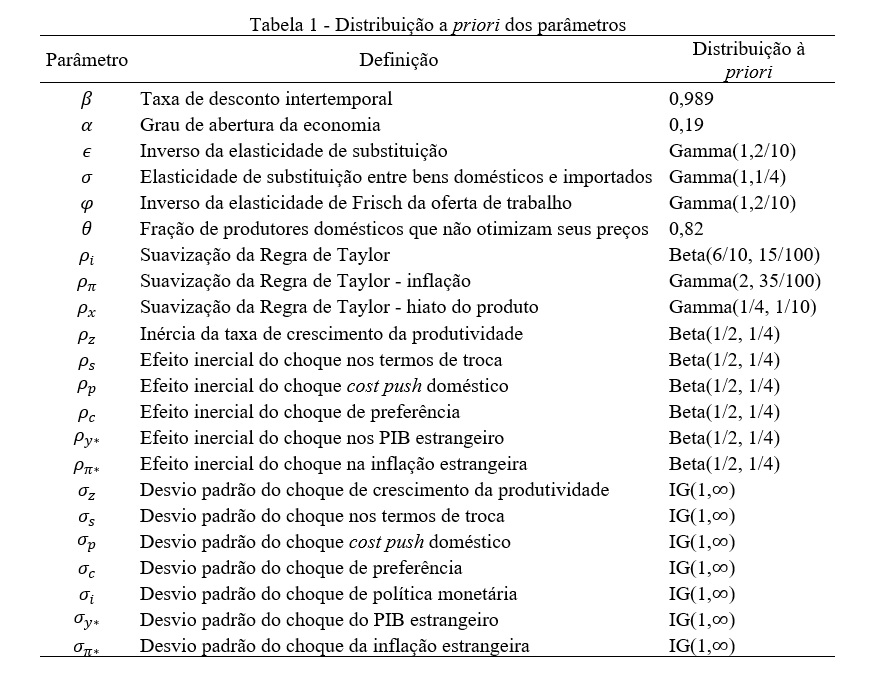
\includegraphics[scale=0.55]{Tabelaprioris.jpg}
%\caption {\tiny Taxa Natural de Juros}
\end{figure}


\end{frame}
%%%%%%%%%%%%%%%%%%%%%%%%%%%%%%%%%%%%%%%%%%%%%%%%%%%%%%%%%%%%%%%%%%%%%%%%%%%%
%%%%%%%%%%%%%%%%%%%%%%%%%%%%%%%%%%%%%%%%%%%%%%%%%%%%%%%%%%%%%%%%%%%%%%%%%%%%
\begin{frame}{Resultados}
\begin{itemize}
    \item Regra de Taylor
\end{itemize}
\begin{figure}[H]
\centering
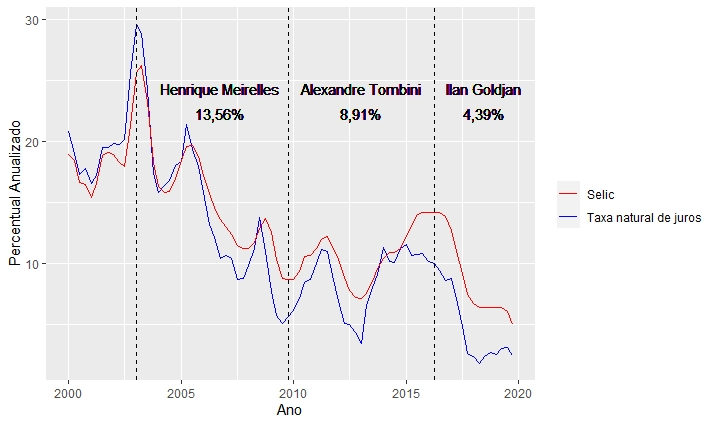
\includegraphics[scale=0.60]{ModeloA.jpeg}
%\caption {\tiny Taxa Natural de Juros}
\end{figure}

\end{frame}
%%%%%%%%%%%%%%%%%%%%%%%%%%%%%%%%%%%%%%%%%%%%%%%%%%%%%%%%%%%%%%%%%%%%%%%%%%%%
%%%%%%%%%%%%%%%%%%%%%%%%%%%%%%%%%%%%%%%%%%%%%%%%%%%%%%%%%%%%%%%%%%%%%%%%%%%%
\begin{frame}{Resultados}
\begin{itemize}
    \item Regra Wickseliana
\end{itemize}
\begin{figure}[H]
\centering
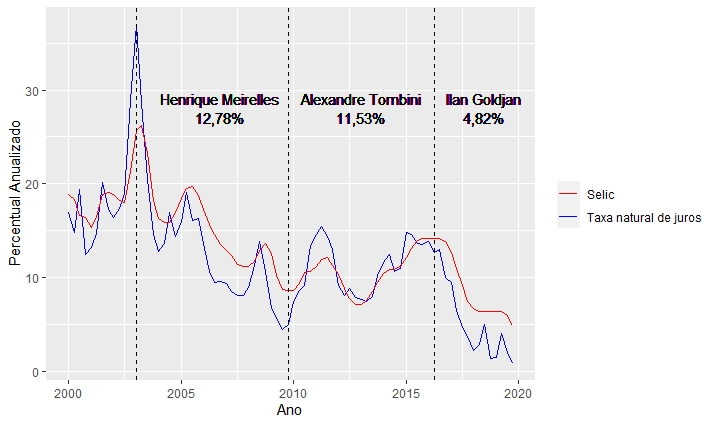
\includegraphics[scale=0.60]{ModeloB.jpeg}
%\caption {\tiny Taxa Natural de Juros}
\end{figure}

\end{frame}
%%%%%%%%%%%%%%%%%%%%%%%%%%%%%%%%%%%%%%%%%%%%%%%%%%%%%%%%%%%%%%%%%%%%%%%%%%%%
%%%%%%%%%%%%%%%%%%%%%%%%%%%%%%%%%%%%%%%%%%%%%%%%%%%%%%%%%%%%%%%%%%%%%%%%%%%%
\begin{frame}{Resultados}
\begin{itemize}
    \item Regra Taylor + Wickseliana
\end{itemize}
\begin{figure}[H]
\centering
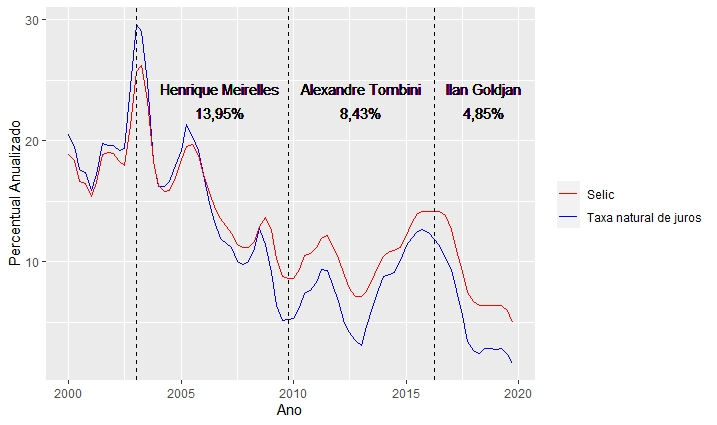
\includegraphics[scale=0.60]{ModeloC.jpeg}
%\caption {\tiny Taxa Natural de Juros}
\end{figure}

\end{frame}
%%%%%%%%%%%%%%%%%%%%%%%%%%%%%%%%%%%%%%%%%%%%%%%%%%%%%%%%%%%%%%%%%%%%%%%%%%%%
%%%%%%%%%%%%%%%%%%%%%%%%%%%%%%%%%%%%%%%%%%%%%%%%%%%%%%%%%%%%%%%%%%%%%%%%%%%%
\begin{frame}{Conclusão}
\begin{itemize}
    \item Taxa natural de juros varia ao longo dos anos e tem apresentado um declínio consistente
    
    \item Resultado se mantem para as três diferentes regras de política monetária
    
    \item Durante a gestão de Henrique Meirelles, o modelo em que o banco central respondia a taxa neutra de juros apresentou a menor média de juros natural 
    
    \item Sob a gestão de Alexandre Tombini, a menor média de taxa neutra foi estimada com a regra de política monetária que combina a regra de Taylor com a Wickseliana 
    
    \item Enquanto Ilan Goldfjan foi presidente do banco central, a menor média de juros neutro foi encontrada quando o BC segui a regra de Taylor
    
\end{itemize}


\end{frame}

%
%
\end{document}
